\chapter{Metodologias}
\label{chap:metodologia}
Nesta seção serão apresentadas as metodologias usadas para o desenvolvimento desse trabalho. As etapas a serem seguidas estão representadas no fluxograma da Figura \ref{fig:etapas}.

\begin{figure}[ht]
  \centering
  \captionsetup{width=16cm}
  \caption{Fluxograma das etapas}
  \label{fig:etapas}
  \tcbox[left=0cm, right=0cm, top=0cm, bottom=0cm,center]{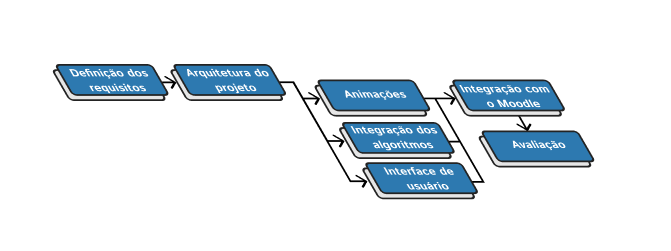
\includegraphics[width=15.6cm]{figuras/fluxograma.png}}
  \Fonte{fornecida pelo próprio autor}
\end{figure}

\section{Definição dos requisitos}
O primeiro passo no desenvolvimento de software é a definição dos requisitos, com eles tem-se um direcionamento sobre o que deve ser feito. A partir da revisão bibliográfica foram definidos alguns requisitos básicos que deveriam estar presentes na ferramenta. Como requisito não funcional foi definido oferecer suporte multi-plataforma, para \textit{mobile}, \textit{desktop} e \textit{web}. Como requisitos funcionais foram definidos os seguintes:
\begin{itemize}[label={$\sbullet$}]
  \item Permitir que os usuários digitem uma gramática para ser analisada.
  \item Permitir que os usuários visualizem o estado das estruturas dos algoritmos.
  \item Permitir que os usuários avancem, retornem e reiniciem os passos da execução dos algoritmos.
  \item Permitir que os usuários selecionem o algoritmo a ser visualizado.
  \item Permitir que os usuários acessem o pseudocódigo dos algoritmos.
  \item Permitir que os usuários adicionem \textit{breakpoints} no pseudocódigo.
  \item Permitir que os usuários visualizem o autômato dos algoritmos LR.
\end{itemize}

Apesar das ferramentas compartilharem as mesmas funcionalidades básicas já definidas inicialmente, outras têm características interessantes que podem ser reaproveitadas, partir delas foram definidos os seguintes requisitos:
\begin{itemize}[label={$\sbullet$}]
  \item Permitir que os usuários digitem uma \textit{string} para ser analisada.
  \item Permitir que os usuários visualizem a análise de uma \textit{string}.
  \item Permitir que os usuários visualizem a árvore sintática de uma \textit{string}.
  \item Permitir que os usuários copiem em formato de texto o resultado dos algoritmos.
\end{itemize}

\section{Definição da arquitetura do projeto}
O projeto será construído usando o \textit{framework Svelte}, sem \gls{ssr}, para que seja possível o funcionamento \textit{offline} da ferramenta, já que a ferramenta não teria acesso ao servidor não seria possível usá-lo para renderizar elementos. \textit{Svelte} compila a base de código e cria uma coleção de arquivos estáticos que constituem a página \textit{web} e a base para o suporte multi-plataforma da aplicação.
\begin{figure}[ht]
  \centering
  \captionsetup{width=16cm}
  \caption{Arquitetura da aplicação em nuvem}
  \label{fig:arqremo}
  \tcbox[left=0cm, right=0cm, top=0cm, bottom=0cm,center]{
    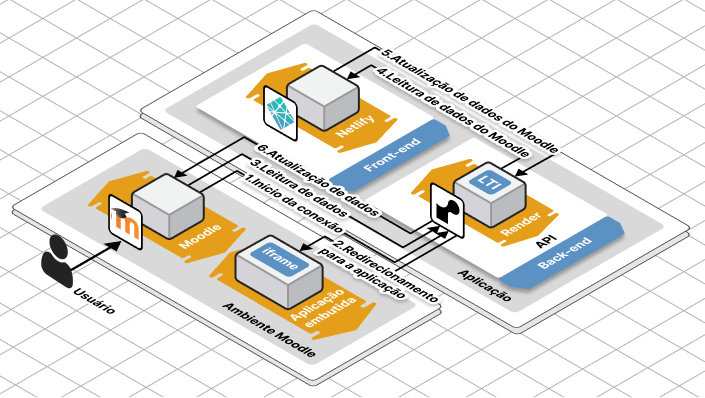
\includegraphics[width=15.6cm]{figuras/remote.png}}
  \Fonte{fornecida pelo próprio autor}
\end{figure}

O \textit{framework Capacitor}\footnote{https://capacitorjs.com} consome essa coleção de arquivos e cria um projeto para plataforma \textit{Android} que é usado para criar a versão \textit{mobile} da ferramenta usando o \textit{Android Studio}. O \textit{framework Tauri}\footnote{https://tauri.app} constrói instaladores para \textit{desktop} diretamente da coleção de arquivos estáticos. A plataforma alvo dos instaladores é a plataforma na qual eles são construídos, já que o \textit{framework} não tem suporte para construção \textit{cross-platform} é necessária a utilização de máquinas virtuais para construir instaladores para diferentes plataformas \textit{desktop}.

Para a versão \textit{online} da aplicação, os serviços  de computação em nuvem \textit{Netlify}\footnote{https://www.netlify.com} e \textit{Supabase}\footnote{https://supabase.com} serão usados para hospedar respectivamente a aplicação e a database usada por ela. \textit{Netlify} e \textit{Supabase} foram escolhidos pela facilidade de uso e pelo oferecimento gratuito dos serviços para aplicações pequenas como a proposta nesse trabalho. O projeto da aplicação foi hospedado em um repositório no \textit{Github}\footnote{https://github.com} que é uma plataforma \textit{web} de hospedagem de repositórios do sistema de versionamento \textit{Git}\footnote{https://git-scm.com}. Graças a integração entre \textit{Netlify} e \textit{Github}, a aplicação é atualizada automaticamente com cada \textit{commit} feito para o repositório do projeto. Por fim, a plataforma \textit{Supabase} será utilizada para armazenar arquivos de \textit{log} da utilização da aplicação durante os testes.

\section{Implementação da interface de usuário}
Nesta seção estão descritos o \textit{layout} da ferramenta e os elementos que o constituem. Começando pela barra de navegação, que contém abas que levam para guias de entrada da gramática e dos algoritmos. A primeira aba é a de entrada da gramática, nessa aba há apenas uma caixa de texto para digitar a entrada. Os elementos descritos nesse parágrafo podem ser vistos na Figura \ref{fig:mgrammar}.

\begin{figure}[ht]
  \centering
  \captionsetup{width=16cm}
  \caption{Aba de entrada da gramática}
  \label{fig:mgrammar}
  \tcbox[left=0cm, right=0cm, top=0cm, bottom=0cm,center]{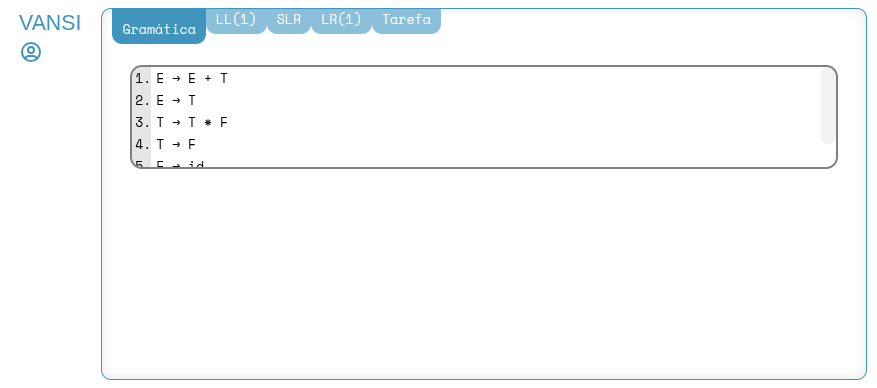
\includegraphics[width=15.6cm]{figuras/mgrammar.png}}
  \Fonte{fornecida pelo próprio autor}
\end{figure}

Na aba dos algoritmos há uma barra de ações com butões separados em dois grupos. No grupo da esquerda, os dois primeiros butões abrem respectivamente uma jenela de diálogo com os resultados em formato de texto e uma janela de diálogo com uma descrição do algoritmo. Os outros dois butões do grupo da esquerda alternam entre a visualização da construção do \textit{parser} e a visualização da análise de uma \textit{string} usando o \textit{parser} construído. No grupo de butões da direita estão os controles de fluxo da execução do algoritmo. O primeiro butão vai para o passo da execução digitado no campo de texto ao lado desse butão, os demais butões realizam as respectivas ações: ir para o passo anterior, reiniciar, ir para o passo seguinte e pular para o fim da execução. Logo abaixo da barra de ações há uma lista de butões, cada um deles abre a visualização de um algoritmo secundário usado na construção do parser selecionado e abaixo desses butões estão os elementos que representam as estruturas de dados dos algoritmos. Os elementos descritos nesse parágrafo podem ser vistos na Figura \ref{fig:malg}.

\begin{figure}[ht]
  \centering
  \captionsetup{width=16cm}
  \caption{Aba de visualização do algoritmo SLR}
  \label{fig:malg}
  \tcbox[left=0cm, right=0cm, top=0cm, bottom=0cm,center]{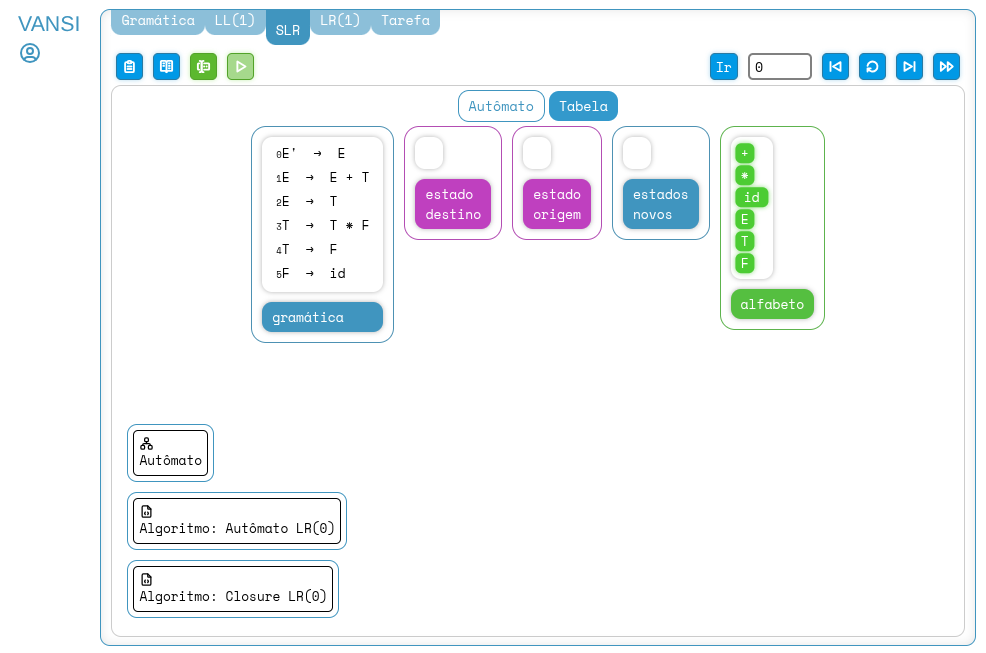
\includegraphics[width=15.6cm]{figuras/malg.png}}
  \Fonte{fornecida pelo próprio autor}
\end{figure}

Ainda na aba dos algoritmos, existem janelas flutuantes onde são mostrados os pseudocódigos dos algoritmos e autômatos. Essas janelas flutuantes são abertas clicando em um botão flutuante com um icóne e título descrevendo a janela. Dentro dessas janelas, no canto superior direito existe uma bandeja de ações com alguns butões. O primeiro butão minimiza a janela, o segundo ativa a ação de mover a janela ao clicar e arrastar ela e o terceiro ativa a interação com a janela. Na janela flutuante que mostra um autômato há um quarto botão na bandeja de ações. Esse botão permite que os estados do autômato sejam movidos. Por fim, nos cantos das janelas flutuantes existem pequenos quadrados que servem para redimensionar a janela. Os elementos descritos nesse parágrafo podem ser vistos na Figura \ref{fig:malgjan}.

\begin{figure}[ht]
  \centering
  \captionsetup{width=16cm}
  \caption{Aba de visualização do algoritmo LR(1)}
  \label{fig:malgjan}
  \tcbox[left=0cm, right=0cm, top=0cm, bottom=0cm,center]{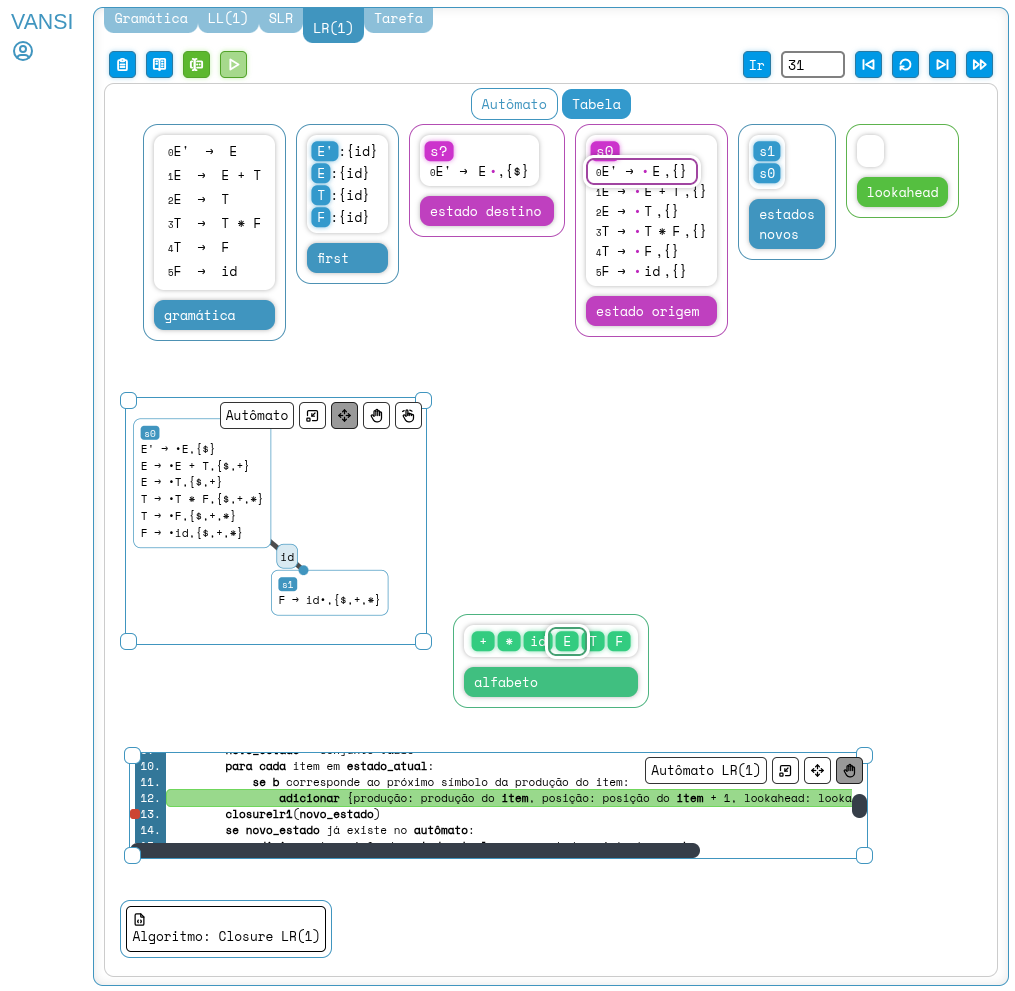
\includegraphics[width=15.6cm]{figuras/malgjan.png}}
  \Fonte{fornecida pelo próprio autor}
\end{figure}

Dentro da aba de análise de \textit{strings}, no lado esquerdo está uma área de visualização da árvore sintática, no lado direito está um campo de texto para digitar a \textit{string} de entrada e logo abaixo estão os elementos que representam as estruturas de dados dos algoritmos. Os elementos descritos nesse parágrafo podem ser vistos na Figura \ref{fig:manalise}.

\begin{figure}[ht]
  \centering
  \captionsetup{width=16cm}
  \caption{Aba de visualização da análise de uma \textit{string}}
  \label{fig:manalise}
  \tcbox[left=0cm, right=0cm, top=0cm, bottom=0cm,center]{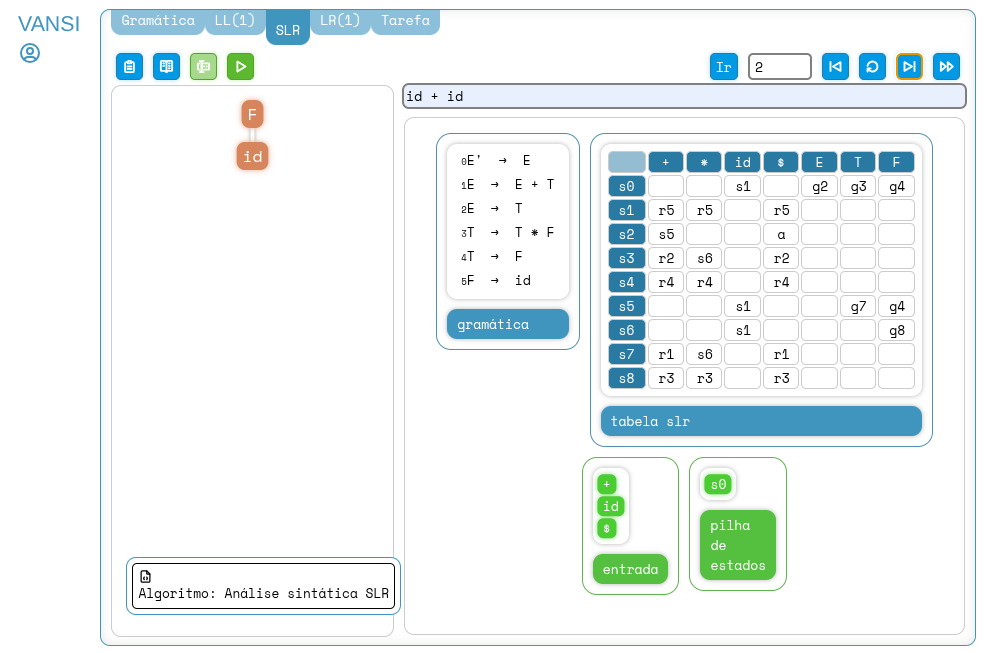
\includegraphics[width=15.6cm]{figuras/manalise.png}}
  \Fonte{fornecida pelo próprio autor}
\end{figure}

As janelas de diálogo aparecem contidas na área de visualização da execução dos algoritmos. Acima de cada janela está um botão de fechar que cobre o comprimento inteiro da janela. Dentro da janela de diálogo para copiar os resultados dos algoritmos em formato de texto estão os resultados de cada algoritmo divididos em seções e ao lado do título de cada seção está um butão de copiar. Na janela de diálogo de descrição do algoritmo tem apenas conteúdo textual. Os elementos descritos nesse parágrafo podem ser vistos na Figura \ref{fig:mpopup}.

\begin{figure}[ht]
  \centering
  \captionsetup{width=16cm}
  \caption{Janela de diálogo para copiar resultados}
  \label{fig:mpopup}
  \tcbox[left=0cm, right=0cm, top=0cm, bottom=0cm,center]{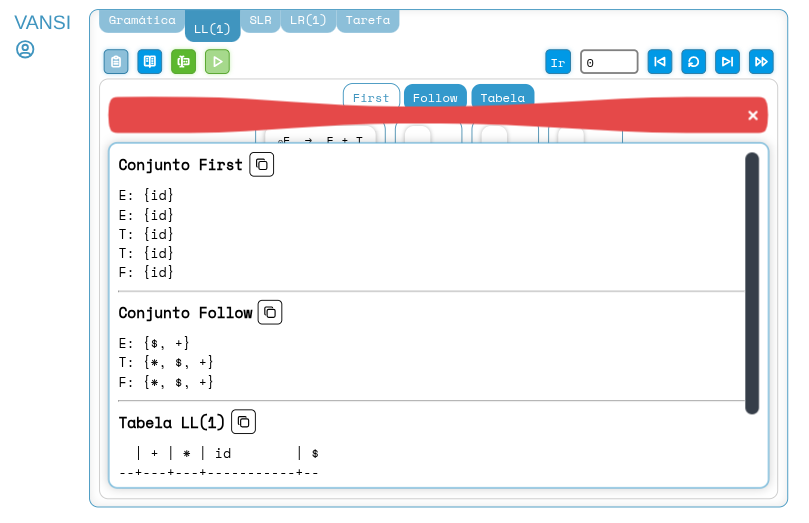
\includegraphics[width=15.6cm]{figuras/mpopup.png}}
  \Fonte{fornecida pelo próprio autor}
\end{figure}

Nas abas de visualização de algoritmos serão inclusos um campo de texto no qual o usuário poderá inserir uma \textit{string} de entrada para ser analisada pelo algoritmo, um campo de texto para copiar os resultados dos algoritmos em forma de texto e um campo de texto para copiar a implementação do algoritmo.

\section{Integração dos algoritmos à ferramenta}
Para todas as estruturas de dados usadas nos algoritmos serão criadas representações visuais, dessa forma todos os passos do funcionamento poderão ser representados como estados dessas estruturas. Calculando antecipadamente os estados dessas estruturas em cada passo dos algoritmos podemos fazer um controle de fluxo entre os passos dos algoritmos.

\section{Implementação das animações dos algoritmos}
As mudanças de estados que ocorrem nos algoritmos podem ser melhor compreendidas se poderem ser visualizadas como transições ao invés de mostrar as mudanças saltando do estado inicial para o estado final. Usar animações torna a visualização das mudanças muito mais dinâmica. Um exemplo de animação é a animação do estado da estrutura de pilha que é usada em alguns algoritmos. Quando um item é adicionado ou removido da pilha, o elemento visual que representa esse item terá sua posição interpolada do ponto inicial ao ponto final.

% \section{Integrar a ferramenta com o \textit{Moodle}}
% A plataforma \gls{lms} \textit{Moodle} implementa o padrão \gls{lti} o que permite a utilização da ferramenta criada nesse trabalho diretamente no \textit{Moodle} sem necessidade de \textit{login} externo. Para que a ferramenta possa utilizar o padrão \gls{lti} com o \textit{Moodle} será implementado no \textit{back-end} da aplicação uma \gls{api} que manuseia as requisições relacionada ao \gls{lti}.

% Os \textit{endpoints} da \gls{api} foram definidos de acordo com o Quadro \ref{qua:endpoints}.

% \setlength{\abovecaptionskip}{10pt plus 0pt minus 0pt}
% \setlength{\belowcaptionskip}{5pt plus 0pt minus 0pt}
% \begin{table}[ht]
%   \centering\setlength{\extrarowheight}{2pt}
%   \captionsetup{width={\textwidth}}
%   \captionof{quadro}{Endpoints}\label{qua:endpoints}
%   \resizebox{\textwidth}{!}{
%     \begin{NiceTabular}{m[c]{3cm}m[c]{3cm}m[c]{10cm}}[corners,hvlines]
%       \CodeBefore
%       \rowcolor{gray!15}{1-1}
%       \Body
%       \textbf{Endpoint}                                                  & \textbf{Método} & \textbf{Finalidade}                 \\
%       \selectlanguage{brazil}$\backslash$\selectlanguage{brazil}         & GET             & redirecionar para página            \\
%       \selectlanguage{brazil}$\backslash$\selectlanguage{brazil}login    & POST            & inicia uma conexão com a plataforma \\
%       \selectlanguage{brazil}$\backslash$\selectlanguage{brazil}register & POST            & registrar uma nova plataforma       \\
%     \end{NiceTabular}}
%   {\Fonte{fornecido pelo autor}}
% \end{table}

% Com a \gls{api} pronta pode ser feita a conexão entre a ferramenta e a \gls{lms}. Utilizando o serviço \gls{lti} de \textit{Dynamic Registration} é possível fazer o cadastro da ferramenta no \textit{Moodle} utilizando um \textit{link} para o \textit{endpoint} de registro dinâmico da \gls{api}.

\section{Avaliação da ferramenta}
Será realizado um teste prático com um grupo de estudantes, onde os eles serão solicitados a realizar tarefas específicas utilizando a ferramenta. Serão coletados dados quantitativos, como tempo de execução das tarefas e taxa de acerto, bem como dados qualitativos por meio de questionários e entrevistas para avaliar a percepção dos estudantes sobre a eficácia da ferramenta. Além disso, a comparação dos resultados obtidos com um grupo de controle que não utiliza a ferramenta ajudará a avaliar o impacto da visualização na compreensão e desempenho dos alunos. Essa abordagem abrangente de avaliação garantirá uma análise completa da eficácia e utilidade da ferramenta desenvolvida nesse trabalho.

O desenvolvimento desse trabalho seguirá o cronograma mostrado no Quadro \ref{qua:cronograma}.
\setlength{\abovecaptionskip}{10pt plus 0pt minus 0pt}
\setlength{\belowcaptionskip}{5pt plus 0pt minus 0pt}
\begin{table}[h]
  \centering\setlength{\extrarowheight}{2pt}
  \captionsetup{width={\textwidth}}
  \captionof{quadro}{Cronograma}\label{qua:cronograma}
  \resizebox{\textwidth}{!}{\begin{NiceTabular}{l*{6}{c}}[corners,hvlines]
      \CodeBefore
      \rowcolor{gray!15}{1-3}
      \Body
      \Block{3-1}{Atividades}             & \Block{1-6}{Período}                                                               \\
                                          & \Block{1-3}{2024}    &          &          & \Block{1-3}{2025}                     \\
                                          & Outubro              & Novembro & Dezembro & Janeiro           & Fevereiro & Março \\

      Definir dos requisitos              & x                    &          &          &                   &           &       \\
      Definir arquitetura do projeto      & x                    &          &          &                   &           &       \\
      Implementar da interface de usuário &                      & x        & x        &                   &           &       \\
      Integrar os algoritmos              &                      &          & x        & x                 & x         &       \\
      Implementar as animações            &                      &          & x        & x                 & x         &       \\
      Integrar ao Moodle                  &                      &          &          & x                 & x         &       \\
      Avaliar a ferramenta                &                      &          &          &                   & x         &       \\
      Escrita do TCC II                   & x                    & x        & x        & x                 & x         & x     \\
      Defesa do TCC II                    &                      &          &          &                   &           & x     \\
    \end{NiceTabular}}
  {\Fonte{fornecido pelo autor}}
\end{table}
